\documentclass[journal,12pt,twocolumn]{IEEEtran}
%
\usepackage{setspace}
\usepackage{gensymb}
\usepackage{xcolor}
\usepackage{polynom}
\usepackage{caption}
%\usepackage{subcaption}
%\doublespacing
\singlespacing

%\usepackage{graphicx}
%\usepackage{amssymb}
%\usepackage{relsize}
\usepackage[cmex10]{amsmath}
\usepackage{mathtools}
%\usepackage{amsthm}
%\interdisplaylinepenalty=2500
%\savesymbol{iint}
%\usepackage{txfonts}
%\restoresymbol{TXF}{iint}
%\usepackage{wasysym}
\usepackage{hyperref}
\usepackage{amsthm}
\usepackage{mathrsfs}
\usepackage{txfonts}
\usepackage{stfloats}
\usepackage{cite}
\usepackage{cases}
\usepackage{subfig}
%\usepackage{xtab}
\usepackage{longtable}
\usepackage{multirow}
%\usepackage{algorithm}
%\usepackage{algpseudocode}
%\usepackage{enumerate}
\usepackage{enumitem}
\usepackage{mathtools}
%\usepackage{iithtlc}
%\usepackage[framemethod=tikz]{mdframed}
\usepackage{listings}

\let\vec\mathbf
\newcommand{\myvec}[1]{\ensuremath{\begin{pmatrix}#1\end{pmatrix}}}

%\usepackage{stmaryrd}


%\usepackage{wasysym}
%\newcounter{MYtempeqncnt}
\DeclareMathOperator*{\Res}{Res}
%\renewcommand{\baselinestretch}{2}
\renewcommand\thesection{\arabic{section}}
\renewcommand\thesubsection{\thesection.\arabic{subsection}}
\renewcommand\thesubsubsection{\thesubsection.\arabic{subsubsection}}

\renewcommand\thesectiondis{\arabic{section}}
\renewcommand\thesubsectiondis{\thesectiondis.\arabic{subsection}}
\renewcommand\thesubsubsectiondis{\thesubsectiondis.\arabic{subsubsection}}

%\renewcommand{\labelenumi}{\textbf{\theenumi}}
%\renewcommand{\theenumi}{P.\arabic{enumi}}

% correct bad hyphenation here
\hyphenation{op-tical net-works semi-conduc-tor}

\lstset{
language=Python,
frame=single, 
breaklines=true,
columns=fullflexible
}



\begin{document}
%

\theoremstyle{definition}
\newtheorem{theorem}{Theorem}[section]
\newtheorem{problem}{Problem}
\newtheorem{proposition}{Proposition}[section]
\newtheorem{lemma}{Lemma}[section]
\newtheorem{corollary}[theorem]{Corollary}
\newtheorem{example}{Example}[section]
\newtheorem{definition}{Definition}[section]
%\newtheorem{algorithm}{Algorithm}[section]
%\newtheorem{cor}{Corollary}
\newcommand{\BEQA}{\begin{eqnarray}}
\newcommand{\EEQA}{\end{eqnarray}}
\newcommand{\define}{\stackrel{\triangle}{=}}
\bibliographystyle{IEEEtran}
%\bibliographystyle{ieeetr}
\providecommand{\nCr}[2]{\,^{#1}C_{#2}} % nCr
\providecommand{\nPr}[2]{\,^{#1}P_{#2}} % nPr
\providecommand{\mbf}{\mathbf}
\providecommand{\pr}[1]{\ensuremath{\Pr\left(#1\right)}}
\providecommand{\qfunc}[1]{\ensuremath{Q\left(#1\right)}}
\providecommand{\sbrak}[1]{\ensuremath{{}\left[#1\right]}}
\providecommand{\lsbrak}[1]{\ensuremath{{}\left[#1\right.}}
\providecommand{\rsbrak}[1]{\ensuremath{{}\left.#1\right]}}
\providecommand{\brak}[1]{\ensuremath{\left(#1\right)}}
\providecommand{\lbrak}[1]{\ensuremath{\left(#1\right.}}
\providecommand{\rbrak}[1]{\ensuremath{\left.#1\right)}}
\providecommand{\cbrak}[1]{\ensuremath{\left\{#1\right\}}}
\providecommand{\lcbrak}[1]{\ensuremath{\left\{#1\right.}}
\providecommand{\rcbrak}[1]{\ensuremath{\left.#1\right\}}}
\theoremstyle{remark}
\newtheorem{rem}{Remark}
\newcommand{\sgn}{\mathop{\mathrm{sgn}}}
\providecommand{\abs}[1]{\left\vert#1\right\vert}
\providecommand{\res}[1]{\Res\displaylimits_{#1}} 
\providecommand{\norm}[1]{\lVert#1\rVert}
\providecommand{\mtx}[1]{\mathbf{#1}}
\providecommand{\mean}[1]{E\left[ #1 \right]}
\providecommand{\fourier}{\overset{\mathcal{F}}{ \rightleftharpoons}}
\providecommand{\ztrans}{\overset{\mathcal{Z}}{ \rightleftharpoons}}
%\providecommand{\hilbert}{\overset{\mathcal{H}}{ \rightleftharpoons}}
\providecommand{\system}{\overset{\mathcal{H}}{ \longleftrightarrow}}
	%\newcommand{\solution}[2]{\textbf{Solution:}{#1}}
\newcommand{\solution}{\noindent \textbf{Solution: }}
\providecommand{\dec}[2]{\ensuremath{\overset{#1}{\underset{#2}{\gtrless}}}}
\numberwithin{equation}{section}
%\numberwithin{equation}{subsection}
%\numberwithin{problem}{subsection}
%\numberwithin{definition}{subsection}
\makeatletter
\@addtoreset{figure}{problem}
\makeatother
\let\StandardTheFigure\thefigure
%\renewcommand{\thefigure}{\theproblem.\arabic{figure}}
\renewcommand{\thefigure}{\theproblem}
%\numberwithin{figure}{subsection}
\def\putbox#1#2#3{\makebox[0in][l]{\makebox[#1][l]{}\raisebox{\baselineskip}[0in][0in]{\raisebox{#2}[0in][0in]{#3}}}}
     \def\rightbox#1{\makebox[0in][r]{#1}}
     \def\centbox#1{\makebox[0in]{#1}}
     \def\topbox#1{\raisebox{-\baselineskip}[0in][0in]{#1}}
     \def\midbox#1{\raisebox{-0.5\baselineskip}[0in][0in]{#1}}
\vspace{3cm}

\title{\LARGE{PINGALA ASSIGNMENTS}}
\author{\normalsize J Sai Sri Hari Vamshi\\ \footnotesize AI21BTECH11014}
\date{}
\maketitle
\tableofcontents
\renewcommand{\thefigure}{\theenumi}
\renewcommand{\thetable}{\theenumi}
\bigskip    

\section{JEE 2019}
\noindent Let $\alpha$ and $\beta$ ($\alpha > \beta$) be the roots of the equation $z^2-z-1=0$. Define,

\begin{align}
	a_n & = \frac{\alpha^n-\beta^n}{\alpha-\beta}, \quad n \ge 1\\
	b_n & = a_{n-1} - a_{n+1}, \quad n \ge 2, \quad b_1 = 1
\end{align}

\noindent Verify the following using a python code.

\begin{enumerate}[label=\thesection.\arabic*,ref=\thesection.\theenumi]
		
	\item
		\begin{align}
	     		\sum_{k=1}^na_k = a_{n+2}-1, \quad n \ge 1
		\end{align}
	
	\solution\\
		Download the Python code using
	
		\begin{lstlisting}
$ wget https://https://github.com/HARI-donk-EY/sig_pros/tree/main/pingala/codes/1_1.py
		\end{lstlisting}
	
		and run it using,
	
		\begin{lstlisting}
$ python3 1_1.py
		\end{lstlisting}
		
		From Fig. \ref{fig:1.1}, both the graphs are similar for $LHS$ and $RHS$.\\ 
		Hence 1.1 is true.

		\begin{figure}[ht]
			\begin{center}
				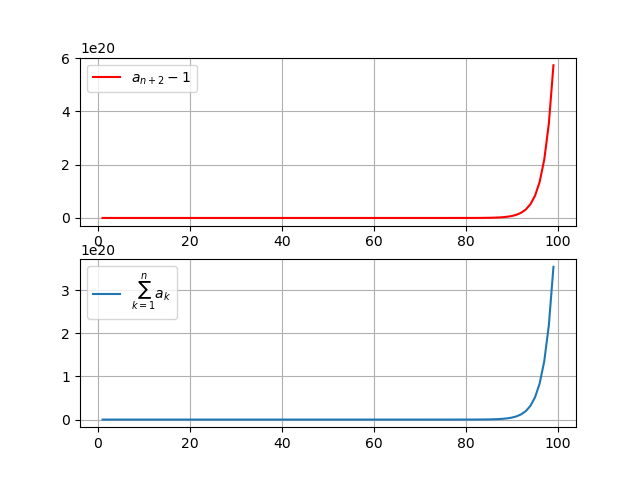
\includegraphics[width=0.7\columnwidth]{figs/1_1}
			\end{center}
			\captionof{figure}{}
			\label{fig:1.1}    
		\end{figure}
			
	\item 
		\begin{align}
	     		\sum_{k=1}^\infty\frac{a_k}{10^k} = \frac{10}{89}
		\end{align}

	\solution
		Download the Python code using
	
		\begin{lstlisting}
$ wget https://https://github.com/HARI-donk-EY/sig_pros/tree/main/pingala/codes/1_2.py
		\end{lstlisting}
	
		and run it using,
	
		\begin{lstlisting}
$ python3 1_2.py
		\end{lstlisting}
		
		The Fig. \ref{fig:1.2} shoes that the difference between $LHS$ and $RHS$ tens to zero as the value of $k$ increases.\\
		It shows that for a large value of $k$, the
		\begin{align*}
			LHS \to RHS	
		\end{align*}
		Hence 1.2 is true.
	
		\begin{figure}[ht]
			\begin{center}
				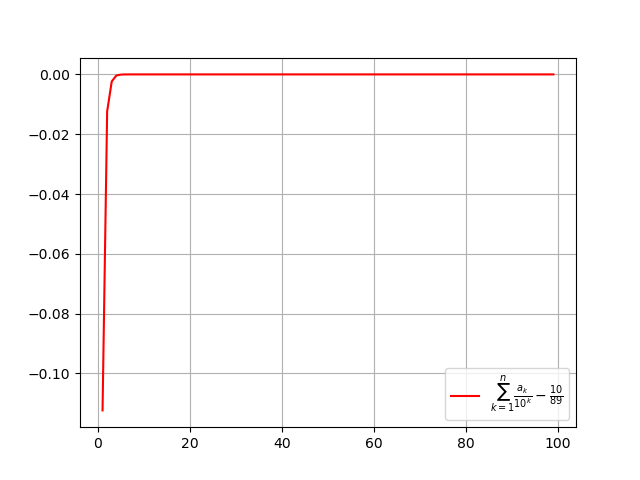
\includegraphics[width=0.7\columnwidth]{figs/1_2}
			\end{center}
			\captionof{figure}{}
			\label{fig:1.2}    
		\end{figure}

	\item 
		\begin{align}
			b_n = \alpha^n + \beta^n, \quad n \ge 1
		\end{align}
	
	\solution	
		Download the Python code using
	
		\begin{lstlisting}
$ wget https://https://github.com/HARI-donk-EY/sig_pros/tree/main/pingala/codes/1_3.py
		\end{lstlisting}
	
		and run it using,
	
		\begin{lstlisting}
$ python3 1_3.py
		\end{lstlisting}
		From Fig. \ref{fig:1.3}, both the graphs are similar for $LHS$ and $RHS$.\\ 
		Hence 1.3 is true.

		\begin{figure}[ht]
			\begin{center}
				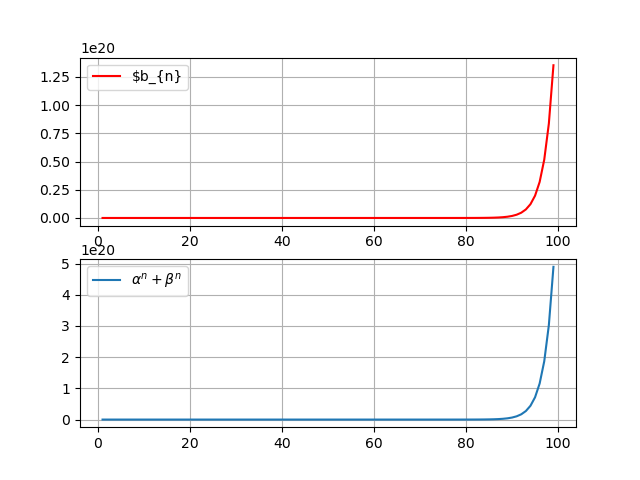
\includegraphics[width=0.7\columnwidth]{figs/1_3}
			\end{center}
			\captionof{figure}{}
			\label{fig:1.3}    
		\end{figure}

	\item 
		\begin{align}
     			\sum_{k=1}^\infty\frac{b_k}{10^k}=\frac{8}{89}
		\end{align}

	\solution\\ 
		Download the Python code using
	
		\begin{lstlisting}
$ wget https://https://github.com/HARI-donk-EY/sig_pros/tree/main/pingala/codes/1_4.py
		\end{lstlisting}
	
		and run it using,
	
		\begin{lstlisting}
$ python3 1_4.py
		\end{lstlisting}
		The Fig. \ref{fig:1.4} shows that the difference between $LHS$ and $RHS$ tends to $\frac{12}{89}$ as the value of $k$ increases.\\
		It shows that for a large value of $k$, the
		\begin{align*}
			LHS \nrightarrow RHS	
		\end{align*}
		Hence 1.4 is false.
	
		\begin{figure}[ht]
			\begin{center}
				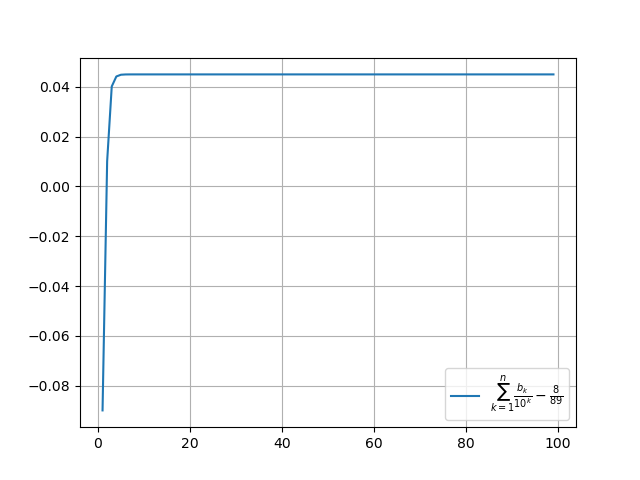
\includegraphics[width=0.7\columnwidth]{figs/1_4}
			\end{center}
			\captionof{figure}{}
			\label{fig:1.4}    
		\end{figure}
\end{enumerate}

\section{Pingala Series}
\begin{enumerate}[label=\thesection.\arabic*,ref=\thesection.\theenumi]
	
	\item The $one\ sided$ $Z$-transform of $x(n)$ is defined as
		\begin{align}
			X^+(z) = \sum_{n=0}^\infty x(n)z^{-n}, \quad z \in \mathbb{C}
			\label{eq:one-Z}
		\end{align}

	\item The {\em Pingala} series is generated using the difference equation  
		\begin{align} 
			x(n+2) = x\brak{n+1} + x\brak{n}\\ 
			x(0) = x(1) = 1, n \ge 0 
			\label{eq:10-pingala} 
		\end{align} 
		Generate a stem plot for $x(n)$.\\

	\solution\\
		Obtain the python code to generate the plot using 
		\begin{lstlisting}
$ wget https://github.com/HARI-donk-EY/sig_pros/tree/main/pingala/codes/2_2.py
		\end{lstlisting}
		Run the code using 
		\begin{lstlisting}
$ python3 2_2.py
		\end{lstlisting}
		The following Fig. \ref{fig:2.2} is obtained
		\begin{figure}[ht]
			\begin{center}
				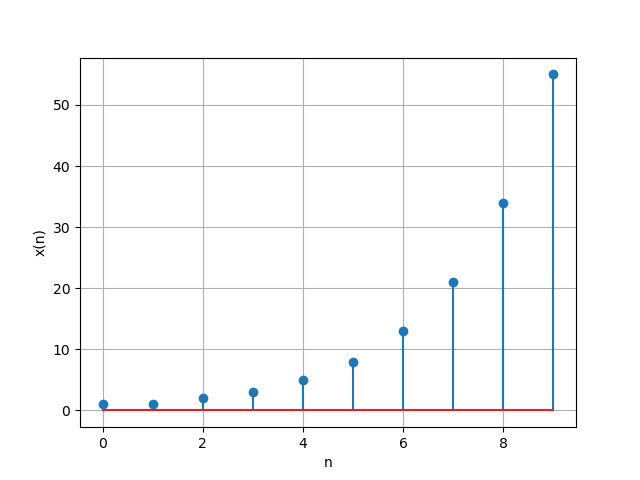
\includegraphics[width=0.7\columnwidth]{figs/2_2}
			\end{center}
			\captionof{figure}{}
			\label{fig:2.2}    
		\end{figure}

	\item Find $X^+(z)$.\\
	\solution\\ 
		\begin{align}
			x(n+2) = x(n+1)+x(n)
		\end{align}
		
		Applying positive $Z$-transform on both sides as w know that $Z$-transform is a linear operator.
		\begin{align}
			\sum_{k=0}^\infty x(k+2)z^{-k} & = \sum_{k=0}^{\infty} x(k+1) + \sum_{k=0}^{\infty} x(k)\\
			z^2\left( X^+(z) - x(0) - x(1) \right) & = X^+(z) + z\left(X^+(z) - x(0)\right)\\
			X^+(z) & = \frac{z^2}{z^2 - z - 1}\\
			X^+(z) & = \frac{1}{1-z^{-1}-z^{-2}}
		\end{align}

	\item Find $x(n)$.\\
	\solution\\
		\begin{align}
			X^+(z) & = \frac{1}{\left(1-\alpha z\right)\left(1-\beta z\right)}
		\end{align}
		
		where $\alpha$, $\beta$ are the roots of the equation
		
		\begin{align}
			z^2 - z - 1 & = 0
		\end{align}

		Co-efficient os $z^{-k}$ in the above expresson is $x(k)$, so by comparing co-efficients.

		\begin{align}
			X^+(z) & = \frac{1}{\alpha - \beta} \left(\frac{\alpha}{1-\alpha z^{-1}} - \frac{\beta}{1-\beta z^{-1}}\right)
		\end{align}

		Using binomial theorem, we get
		\begin{align}
			x(k) & = \frac{\alpha^{k+1} - \beta^{k+1}}{\alpha - \beta}
		\end{align}

	\item Sketch
		\begin{align}
			y(n) & = x(n-1) + x(n+1), \quad n \ge 0
			\label{eq:y_n}
		\end{align}
	\solution\\
		Obtain the python code to generate the plot using 
		\begin{lstlisting}
$ wget https://github.com/HARI-donk-EY/sig_pros/tree/main/pingala/codes/2_5.py
		\end{lstlisting}
		Run the code using 
		\begin{lstlisting}
$ python3 2_5.py
		\end{lstlisting}
		The following Fig. \ref{fig:2.5} is obtained
		\begin{figure}[ht]
			\begin{center}
				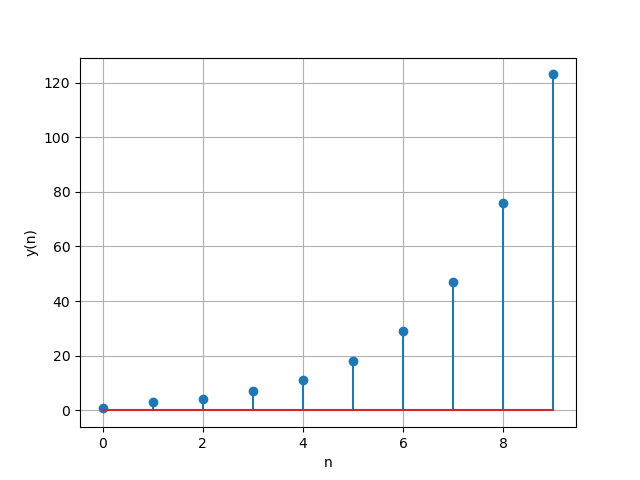
\includegraphics[width=0.7\columnwidth]{figs/2_5}
			\end{center}
			\captionof{figure}{}
			\label{fig:2.5}    
		\end{figure}
		

	\item Find $Y^{+}(z)$.
	\solution\\
		Take +ve $Z$-transform on both sides of \eqref{eq:y_n}.
		\begin{align}
			\sum_{k=0}^{\infty}y(k)z^{-k} & = \sum_{k=0}^{\infty}x(k+1)z^{-k} + \sum_{k=0}^{\infty}z^{-k}\\
			Y^+(z) & = z\left(X^+(z) - x(0)\right) + z^{-1}X^+(z)\\
			\because x(-1) = 0 & \nonumber \\
			Y^+(z) & = \frac{z+z^{-1}}{1-z^{-1}-z^{-2}}-z\\
			\therefore Y^+(z) & = \frac{1+2z^{-1}}{1-z^{-1}-z^{-2}}
		\end{align}

	\item Find $y(n)$.

	\solution\\
		Co-efficient of $z^{-n}$ in $Y^+(z)$ will be $y(n)$.

		\begin{align}
			Y^+(z) & = \frac{1}{1-z^{-1}-z^{-2}} + \frac{2z^{-2}}{1-z^{-1}-z^{-2}}\\
			y(k) & = \frac{\alpha^{k+1} - \beta^{k+1}}{\alpha - \beta} + 2\frac{\alpha^{k} - \beta^{k}}{\alpha - \beta}\\
			y(k) & = \frac{\alpha^{k+2} + \alpha^k - \beta^k - \beta^{k+2}}{\alpha - \beta}\\
			y(k) & = \frac{\alpha^{k+2} - \beta\alpha^{k+1} + \alpha\beta^{k+1} - \beta^{k+2}}{\alpha - \beta}\\
			[\because \alpha\beta = -1]\ & \nonumber\\
			\therefore y(k) & = \alpha^{k+1} + \beta^{k+1}
		\end{align}

\end{enumerate}

\section{POWER OF THE Z TRANSFORM}
\begin{enumerate}[label=\thesection.\arabic*,ref=\thesection.\theenumi]
	
	\item Show that.
		\begin{align}
			\sum_{k=1}^{n} a_k = \sum_{k=0}^{n-1} = x(n) * u(n-1)
		\end{align}
	\solution\\
		\begin{align}
			& x(k) = a(k+1)\\
			& \implies \sum_{k=0}^{n-1} x(k) = \sum_{k=0}^{n-1} a(k+1)\\
			& \implies \sum_{k=1}^{n} a_k = \sum_{k=0}^{n-1} x(k)\\
			& x(n) * u(n-1) = \sum_{k=-\infty}^{\infty} x(k)u(n-k-1)\\
			& u(n-k-1) = 
			\begin{cases}
				0 & k < n-1\\
				1 & k \ge n-1
			\end{cases}\\
			& x(k) = 0, \quad \forall k < 0\\
			& \therefore \sum_{k=0}^{n-1} x(k) = x(n) * u(n-1)
		\end{align}
	
	\item 
		show that,
		\begin{align}
			a_{n+2} -1, \quad n \ge 1
		\end{align}
		can be expressed as,
		\begin{align}
			[x(n+1) -1]u(n)
		\end{align}
	\solution\\
		\begin{align}
			x(k) & = a(k+1) \\ 
			\implies xk+1) & = a(k+2)\\
			a(k+2) -1 & = x(k+1)-1 \\
			\therefore a(k+2)-1 & = [x(k+2)  -1]u(k) \\
			[\because \forall \ \ n \ge 1]
		\end{align}

	\item 
		show that,
		\begin{align}
			\sum_{k=1}^{\infty}\frac{a_k}{10^k} = \frac{1}{10}\sum_{x(k)}^{10^k} = \frac{1}{10}X^+(10)
		\end{align}
	\solution\\
		\begin{align}
			X^{+}(z) & =\sum_{k=0}^{\infty} x(k)z^{-k}=z\sum_{k=1}^{\infty} a(k) z^{-k}\\
			z & =10\\
			\implies 10\sum_{k=1}^{\infty}\frac{a_k}{10^k} & =\sum_{k=0}^{\infty}\frac{x\brak{k}}{10^k}\\ & =X^{+}\brak{{10}}\\
			\sum_{k=1}^{\infty}\frac{a_k}{10^k} & = \frac{1}{10}\sum_{k=0}^{\infty}\frac{x\brak{k}}{10^k}\\
			\therefore \sum_{k=1}^{\infty}\frac{a_k}{10^k} & = \frac{1}{10}X^{+}\brak{{10}}
		\end{align}\\
	
	\item 
		Show that,
		\begin{align}
			\alpha^n + \beta^n, \quad n \ge 1
		\end{align}
		can be expressed as
		\begin{align}
			w(n) =\brak{\alpha^{n+1} + \beta^{n+1}}u(n)
		\end{align}
		and find $W(z)$.\\ \ \\
	\solution\\ \ \\
		Applying Z-transform on both sides,
		\begin{align}
			W(z)&=\sum_{n=-\infty}^{\infty}\brak{\alpha^{n+1} + \beta^{n+1}}u(n)z^{-n}\\
			&=\sum_{n=0}^{\infty}\brak{\alpha^{n+1} + \beta^{n+1}}z^{-n}\\
			&=\alpha \sum_{n=0}^{\infty}(\alpha z^{-1})^{n}+\beta \sum_{n=0}^{\infty} (\beta z^{-1})^{n}\\
			\text{ROC:} & \quad |z|>\text{max}(\alpha,\beta) \nonumber \\
			&=\frac{\alpha}{1-\alpha z^{-1}}+\frac{\beta}{1-\beta z^{-1}}\\
			&=\frac{1+2z^{-1}}{1-z^{-1}-z^{-2}}
		\end{align}

		\item 
			Show that 
			\begin{align}
				\sum_{k=1}^{\infty}\frac{b_k}{10^k} =
				\frac{1}{10}\sum_{k=0}^{\infty}\frac{y\brak{k}}{10^k} =\frac{1}{10}Y^{+}\brak{{10}}
			\end{align}
		\solution\\
			\begin{align}
				y(k)&=b(k+1)\\
				\sum_{k=0}^{\infty} y(k) z^{-k}&=\sum_{k=0}^{\infty} b(k+1) z^{-k}\\ &=Y^{+}(z)\\
				\sum_{k=0}^{\infty} y(k) z^{-k}&=z\sum_{k=1}^{\infty} b(k) z^{-k}\\ &=Y^{+}(z)\\
				\text{Assume:}& \quad z=10\\
				\therefore \sum_{k=1}^{\infty}\frac{b_k}{10^k} & =
				\frac{1}{10}\sum_{k=0}^{\infty}\frac{y\brak{k}}{10^k}\\ &=\frac{1}{10}Y^{+}\brak{{10}}
			\end{align}
	
		\item 
			Solve the JEE 2019 problem.\\
		\solution\\
			1.2\\
			\begin{align}
				X^{+}(z) & =z\sum_{k=1}^{\infty} a(k) z^{-k}\\ & =\frac{1}{1-z^{-1}-z^{-2}}\\ \ \nonumber \\
				\text{Assume:}& \quad z=10\\
				\sum_{k=1}^{\infty} \frac{a_k}{10^k} & =\frac{1}{10 \left(1-\frac{1}{10}-\frac{1}{100}\right)}\\
				&=\frac{10}{89}
			\end{align}
			1.3\\
			\begin{align}
				y(k) & =\alpha^{k+1}+\beta^{k+1}\\
				y(k) & =b(k+1)\\
				\implies b(k) & =\alpha^{k}+\beta^{k}
			\end{align}
			1.4\\
			\begin{align}
				\sum_{k=1}^{\infty}\frac{b_k}{10^k} & = \frac{1}{10}Y^{+}\brak{{10}}\\
				&=\frac{1}{10}\left[\frac{1+\frac{2}{10}}{1-\frac{1}{10}-\frac{1}{100}}\right]\\
				\because Y^{+}(z) & =\frac{1+2z^{-1}}{1-z^{-1}-z^{-2}}\\
				&=\frac{12}{89}
			\end{align}
			Run the following code to get the expressions of $x(n)$ and $y(n)$
			\begin{lstlisting}
$ https://github.com/HARI-donk-EY/sig_pros/tree/main/pingala/codes/Xz.py
			\end{lstlisting}
			Use the following command in the terminal to run the code
			\begin{lstlisting}
$ python3 Xz.py
			\end{lstlisting}

\end{enumerate}

\end{document}

